% Intro text here; a sentence or two (I don't think it's necessary)
\subsection{Q-Learning}

Reinforcement learning seeks to find the optimal action to be undertaken for a given state through trial and error. In the context of Fido, an action could be the playing of a note or driving straight forwards, while the state could be the amount of light detected by the robot or how near the robot is to another object. Once an action is performed, a reward and a new state are given back to the reinforcement learning algorithm.  As actions are performed over time, the reinforcement learning algorithm sharpens its ability to receive reward.

$Q$-Learning \cite{watkins} is a popular reinforcement learning algorithm that works by learning an action-value function $Q$ that takes a state-action pair as an input and outputs the expected utility value of performing that action in that state. This utility value is know as the $Q$-value. The $Q$-value is a combination of immediate reward and expected future reward. Every reward iteration the $Q$-value of an state-action pair is updated as such:

\begin{equation}
	Q(s, a) := Q(s, a)(1 - \alpha) + \alpha(R + \gamma \max Q(s_{t+1}, a))
	\,,
	\label{equ::updateqlearn}
\end{equation}

\noindent
where $a$ is the action carried out, $s$ is the initial state, $R$ is the reward received, and $s_{t+1}$ is the new state. $\alpha$ is the learning rate of the algorithm. The learning rate determines the rate of convergence by diminishing or amplifying the changes made to the $Q$-value each reward iteration. $\gamma$ is the devaluation factor, which determines the weight given to future rewards. A devaluation factor approaching $\gamma=0$ will force the algorithm to only value immediate reward, while a devaluation factor approaching $\gamma=1$ will make it focused on high long term reward.

The $Q$-Learning algorithm had to be immediately modified in two ways to make it suitable for Fido. Its scalability had to be improved, and it had to be able to work in continuous state-action spaces.   

$Q$-learning in its simplest form uses a table to model the $Q$ function, storing past state-action pairs and each pair's respective $Q$-value.  However, this strategy lacks scalability. Since Fido will have to continue to learn throughout its whole lifetime, requiring it to store a large number of $Q$-values, this strategy is rendered impractical. To allow Fido to incorporate a large amount of data into its model of $Q$ while keeping latency low, it is necessary to use a function approximator to estimate $Q$.  Feed-forward neural networks were chosen for this task for their ability to model non-linear functions, lightweight computational footprint, and high trainablility.

Conventional $Q$-Learning is discrete. No relation is made between states or actions, and every action for each state must be performed individually in a noisy feedback system to determine its $Q$-value. However, Fido will work in a large, continuous state-action spaces where relations made between (state-action, $Q$-value) pairs can drastically reduce the number of reward iterations needed for convergence. An example of a task that would benefit from continuity is teaching Fido to adjust the speed of its motors based on the intensity of light that the robot detects. There is an obvious gradient relation between the (state-action, $Q$-value) pairs in this task and with a limited number of $Q$-values known, it is possible to correctly model $Q$.

\subsection{Wire-Fitted Q-Learning}

To accommodate continuous action-spaces, we coupled a wire-fitted moving least squares interpolator with our feed-forward neural network as described in \cite{gaskett}. 

Feed-forward neural networks can generalize between states in $Q$-Learning problems with discrete actions as described in \cite{rummery}. To extend this implementation to a continuous action space, our feed-forward neural network outputs discrete ``wires'' when given a state. Each wire consists of an action with its respective $Q$-value for the state given to the neural network. These wires may be interpolated to model $Q$, allowing us to get the $Q$-value of any action performed in a state given as an input to the network. The interpolator used in Fido is a wire-fitted moving least squares interpolator used in the context of a memory-based learning system \cite{baird}.

The wire-fitting function calculates $Q$-value of an action $\hat{a}$ for a state $s$ given a set of $n$ actions $a$ each with a respective $Q$-value $q$ as such:

\begin{equation}
	Q(a, s) = \cfrac{\sum_{i=0}^{n}\cfrac{q_i}{||\hat{a}-a_i||^2+c(q_{max}-q_i)+k}}{\sum_{i=0}^{n}\cfrac{1}{||\hat{a}-a_i||^2+c(q_{max}-q_i)+k}}
	\,,
\end{equation}

\noindent
where $q_{max}$ is the greatest $Q$-value among the set of $Q$-values $q$, and $k$ is a small value that avoids division by zero. $c$ is the smoothing factor. The greater the smoothing factor, the smoother the interpolated function.


Figure \ref{fig::wirefitexample} is an example of interpolation on a set of wires. The graph shows the value of one-dimensional actions plotted against their respective $Q$-values. The wire-fitting function has few properties that make it especially suited for Fido.

\begin{figure}[ht]
    \centering
    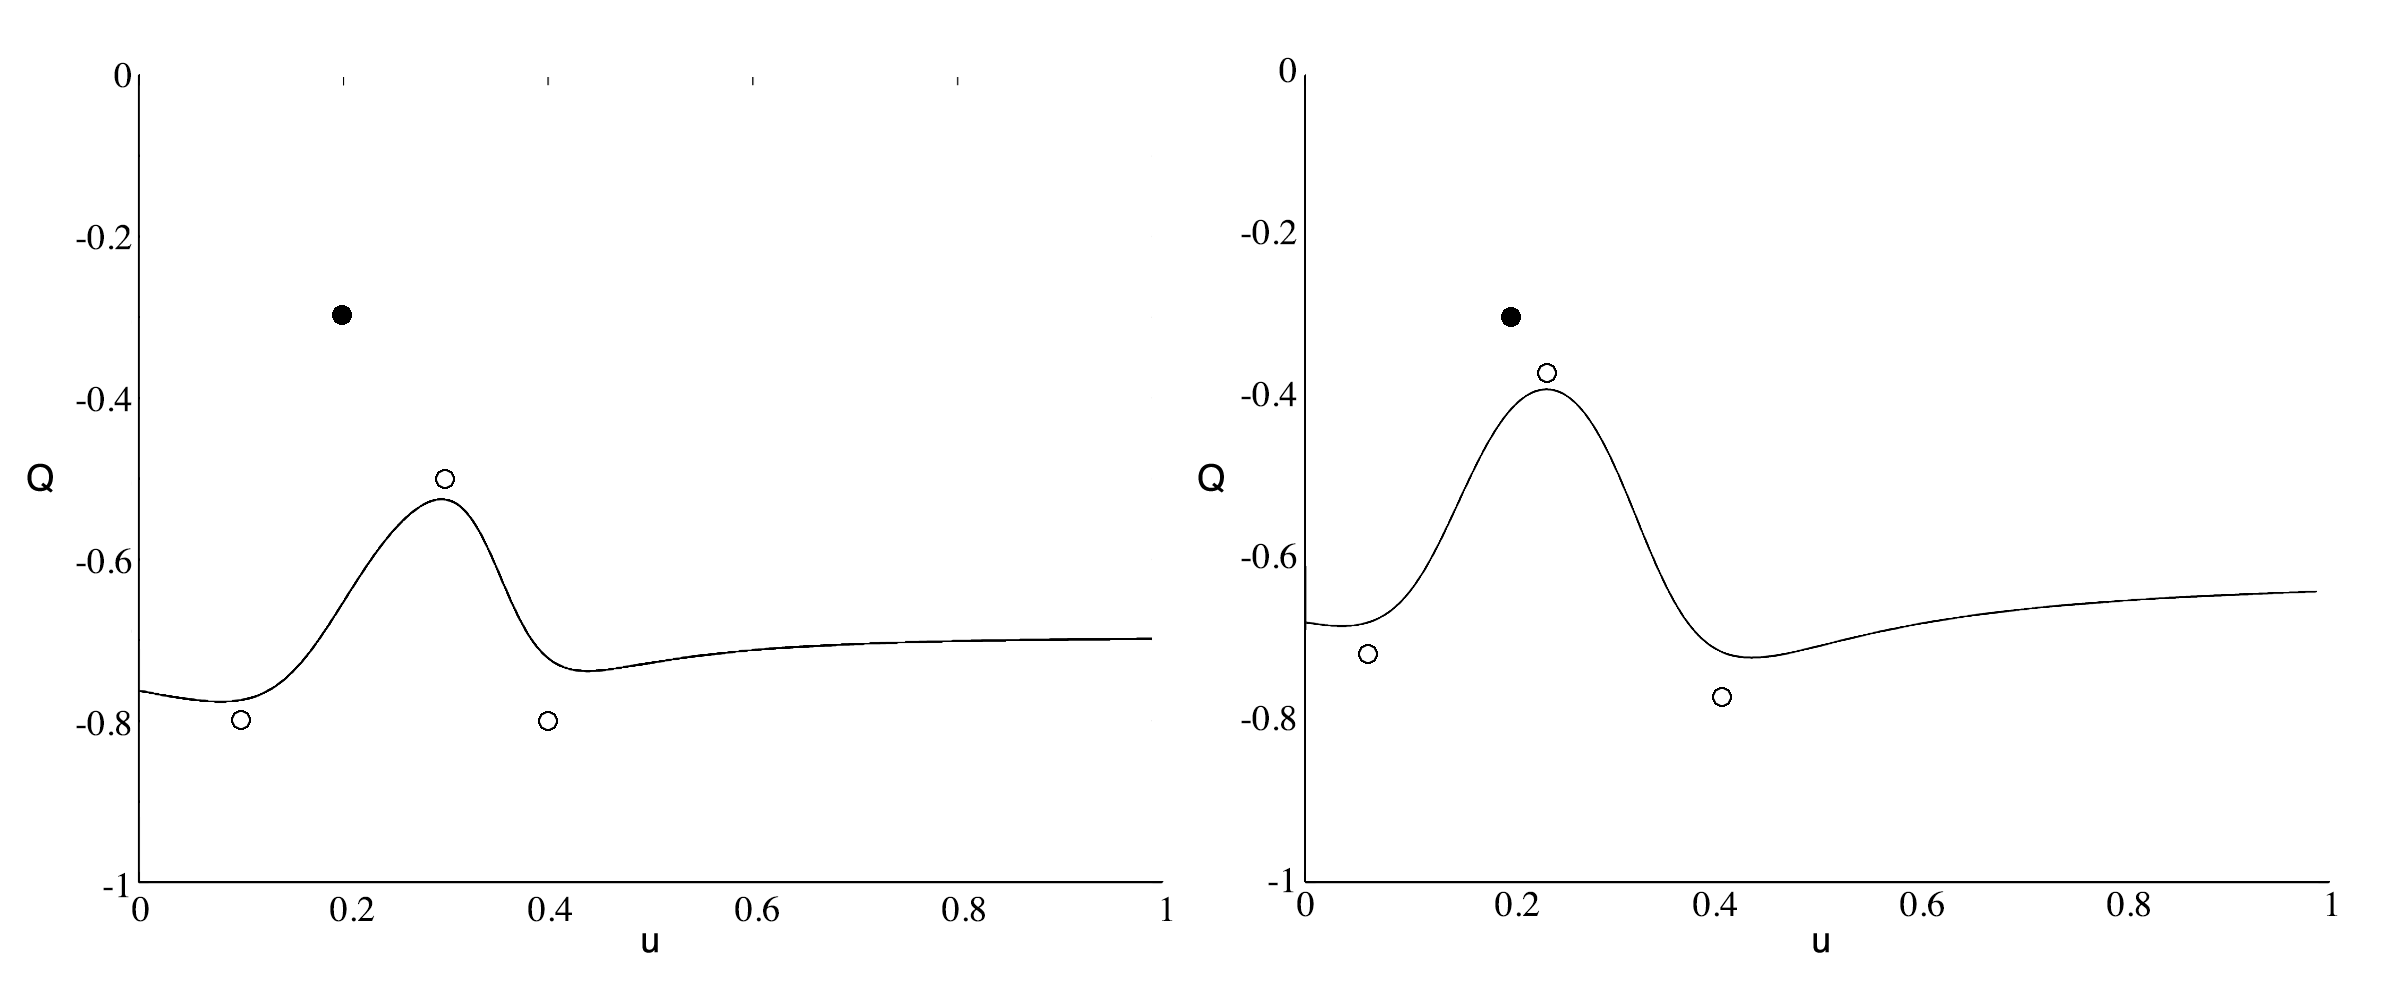
\includegraphics[height=6.5cm]{Figures/WireFit.png}
	\caption{Moving Least Squares Interpolator (adapted from Gaskett, Wettergreen, \& Zelinsky, 1999)}
    \label{fig::wirefitexample}
\end{figure}

Every update to the $Q$-value requires that $q_{max}$ is computed and the action that produces $q_{max}$ is needed for common action selection policies. As proved in \cite{baird}, the wire with the greatest $Q$-value is the interpolation point with the greatest $Q$-value, therefore $q_{max}$ is the maximum $Q$-value out of the set of wires given to the wire-fitting function. This makes it extremely computationally cheap to compute $Q$-value, allowing Fido's latency to stay minimal.

The wire-fitting function is derivable. This allows us to update our wires, and therefore our model of $Q$, using gradient descent. Gradient descent is an optimization algorithm that looks to find the local minimum of a function by modifying each of its parameters, one by one. The update function for a parameter is calculated as such:

\begin{equation}
	a = a - \gamma \Delta F(a)
	\,,
	\label{equ::wirefiterrorfunction}
\end{equation}

where $a$ is the parameter to be updated, $\gamma$ is the learning rate, and $\Delta F(a)$ is the partial derivative of the function to be minimized $F$ with respect to $a$. In the case of Fido, once the reward and new state for an action-state pair is received and an updated $Q$-value $\hat{q}$ is calculated using Equation \ref{equ::updateqlearn}, we are trying to minimize the wire-fitting function's error at predicting $\hat{q}$ when given the wires for Fido's previous state. This error can be calculated as:

\begin{equation}
	(\hat{q} - q)^2
	\,,
	\label{equ::wirefiterrorfunction}
\end{equation}

\noindent

where $q$ is the old $Q$-value. Using Equation \ref{equ::wirefiterrorfunction} as our function to be minimized and the partial derivative of the wire-fitting function with respect to each action vector and each q-value, we may compute the partial derivatives of our cost function. Using these, new wires may be calculated for Fido's previous state using gradient descent. Fido's neural network may be trained using back propagation to output these new wires when given the previous state.

\subsection{Boltzmann Probability Distribution Selection Policy}

$Q$-learn requires that actions are selected to be performed. There are a number of approaches to choosing this action, and each has a large affect on the behavior of the learning implementation. The most common approach is to simply pick the action with the best $Q$-value for the current state. However this strategy stifles exploration of the state-action space, increasing the time of convergence on a task, hurting the retrain-ability of the model, and giving a bias towards an actor's starting policy, which is random. This problem is compounded in the case of Fido due to the large state and action spaces that Fido must explore. Another common method of action selection is to choose each action randomly for a set number of reward iterations, and then to switch to choosing the action with the highest $Q$-value. This plan improves upon the first by allowing for a period of exploration, but is not suited for Fido. During its lifetime, Fido must have the ability to learn new tasks and be retrained by the operator providing feedback, and so, must continuously explore its state space.

Fido selects actions probabilistically using a Boltzmann or soft-max distribution of probability. The likelihood that an action $\hat{a}$ will be chosen from a set of $n$ actions $a$ for a state $s$ is given as:

\begin{equation}
	p(\hat{a}) = \cfrac{e^{\frac{Q(s, \hat{a})}{T}}}{\sum_{i=0}^{n}e^{\frac{Q(s, a_i)}{T}}}
	\,.
	\label{equ::boltzmann}
\end{equation}

$T$ is the temperature, or exploration level. As $T$ approaches infinity, a random action is chosen. As $T$ tends toward 0, the best action is chosen. Fido keeps $T$ at a constant value around $T \approx 0.15$ throughout its lifetime to encourage occasional, continued exploration.